\chapter{Módszertan} 
\label{ch:methodology}

Ebben a fejezetben az alkalmazott módszertant mutatom be. Először ismertetem az alkalmazott előfeldolgozási módszereket. Ezután a tanító modellek architektúráját mutatom be. Végül pedig szót ejtek az ismertetett módszerek implementációjáról.

\section{Bemeneti adatok, előfeldolgozás}

Az OpenMIC adathalmazzal két formában kapjuk meg a bemeneti adatokat. Egyrészt elérhetőek a nyers hanganyagok .ogg formátumban. Ezen kívül rendelkezésre állt a VGGish nevű reprezentáció is, amelyről a korábbi \ref{subsec:VGGish} fejezetben írtam. A bemeneti adatokat tanítás előtt azonban néhány előfeldolgozási folyamaton vittem végig részben a megvalósíthatóság, részben pedig a performancianövelés érdekében. Ezekről írok a következő alfejezekben.

\subsection{Alternatív reprezentációk kinyerése}

A .ogg fájlokból beolvasott nyers audioval való tanítás sajnos nem volt lehetséges, mivel ez egy memória szempontjából igen költséges reprezentáció, amihez a hardver eszközöm kapacitása kevésnek bizonyult. Helyette a dolgozat korábbi fejezetében bemutatott melspectogram és MFCC reprezentációkat használtam fel. Mindkét reprezentációt a beolvasott nyers hullámforma reprezentációból nyertem ki az elméleti háttér fejezetben leírt módon.

\subsection{Adathalmazok normalizálása}

Az adatok normalizálása a tanulási folyamat gyorsítására szolgál. A normalizálást úgy érjük el, hogy az adatokat arányosan a 0 és 1 értékek közé transzformáljuk. Erre egy szokásos megoldás:
\begin{equation}
x(_i) := (x(_i) - x_{\text{min}}) \/ (x_{\text{max}} - x_{\text{min}})
\end{equation}

A normalizált adathalmon a gradiens általában hamarabb csökkenthető, ezért a tanítási folyamat rövidebb lehet. \cite{LeCun2012}

\subsection{Osztályok kiegyensúlyozása}

Tanító modelleknél gyakori probléma, hogy a tanulni kívánt osztályok egy része alul van reprezentálva. Dolgozatom multi-label osztályozása esetén két osztályról beszélhetünk: igaz (jelen van az adott hangszer) és hamis (nincs jelen az adott hangszer). Mivel sok esetben a hamis értékek jelentős többségben voltak, - egyes hangszerek esetén az összes adat közel 80\%-át is kitette - ezért a modell jó pontosságot tudott elérni csupán ''hamis'' predikciókkal.

Ezt elkerülendő, három megoldás jöhetett szóba:
\begin{itemize}
 \item \textbf{Alulmintavételezés (Undersampling)} - a többségi osztályokból véletlenszerűen eltávolítunk annyi elemet, hogy az osztályok kiegyensúlyozottá váljanak.
 \item \textbf{Túlmintavételezés (Oversampling)} - a kisebbségi osztályok véletlenszerű elemeit duplikáljunk addig, amíg az osztályok kiegyensúlyozottá válnak.
 \item \textbf{Adat augmentáció (Data augmentation)} - hasonlóan az oversampling technikához a kisebbségi osztály elemeit bővítjük. Ebben az esetben a meglévő elemek transzformálásával mesterségesen hozunk létre új elemeket (pl. képeknél forgatás). \cite{imbalanced}
\end{itemize}

Dolgozatom keretében az undersampling módszert alkalmaztam.

\subsection{Tanító-, tesztelő- és validáló halmaz kialakítása}

Tanító modellek alkalmazásakor fontos, hogy legalább kettő, de inkább három független adathalmazzal rendelkezzünk: 
\begin{itemize}
 \item \textbf{Tanító adathalmaz (Train Set)} - ebből a halmazból tanul és ezt a halmazt látja a modellünk.
 \item \textbf{Validáló adathalmaz (Validation Set)} - a tanítási lépések (epoch-ok) között ezen a tanító halmaztól független adathalmazon kiértékeljük modellünk működését. Ezáltal visszajelzést tudunk adni a tanítási folyamat felé és ha szükséges, változtathatunk a hiperparamétereken. Modellünk tehát ezt a halmazt időnként látja, de nem ebből tanul
 \item \textbf{Teszt adathalmaz (Test Set)} - a tanítási folyamat végén ezen a halmazon értékeljük ki modellünk teljesítményét. Modellünk ezt a halmazt a tanítás alatt egyáltalán nem látja és ezáltal nem is tud tanulni belőle. Ezzel a függetlenséggel biztosítjuk a kiértékelés torzítatlanságát. \cite{traintestvalid}
\end{itemize}

Bevett szokás, hogy e három halmazt körülbelül 60\%-20\%-20\% arányban osztjuk fel a tanító halmaz javára. \cite{traintestvalid} Dolgozatom során én is ezt az elvet követtem.

\section{Architektúra}

A következő alfejezetekben a különböző tanító modell kísérletek architektúráját mutatom be.

\subsection{Hagyományos Machine Learning (Modeling Baseline)}

Az OpenMIC dataset megalkotói bemutattak egy példa modellt, amely egy véletlen erdő osztályozó (Random Forest Classifier). \cite{humphrey2018openmic} Ez egy hagyományos gépi tanulási algoritmus. Az osztályozó 100 eldöntési fából áll, a maximális mélysége 8. Ez szolgált munkám kiinduló pontjaként. A továbbiakban Modeling Baseline elnevezéssel hivatkozok rá.

A Modeling Baseline futtatását alapvetően a VGGish reprezentációra implementálták. Dolgozatom keretében megvalósítottam ugyanennek az osztályozónak a melspectogram, ileltve MFCC reprezentációkon való tanítását is. Ezáltal minden reprezentációra kaptam egy viszonyítási alapot.

\subsection{Deep CNN}

Az első mély tanulási megközelítésem a VGG-16 \cite{vgg} architektúrához hasonló mély konvolúciós neuronháló megvalósítása. Ennek megfelelően Deep CNN néven fogok rá hivatkozni a továbbiakban. A VGG-16 egy 2014-ben bemutatott architektúra, amelyet 224x224 méretű RGB képek tanítására hoztak létre. Több tanulmány is azt állítja, hogy az ehhez hasonló mély konvolúciós hálók hangok tanítására is alkalmasak lehetnek (például \cite{choi2017tutorial}). Erre az állításra az intuíció pedig az lehet, hogy a hangok különböző kétdimenziós reprezentációi képek, melyekben a mély konvolúciós hálók mintákat, összefüggéseket tudnak keresni.


\begin{figure}[H]
  \centering
  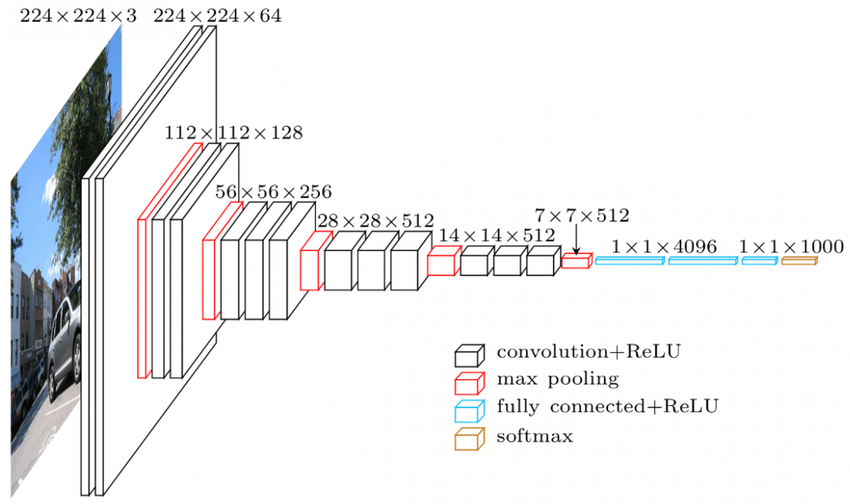
\includegraphics[width=\textwidth, height=8cm]{vgg.png}
  \caption{VGG-16 neurális háló architektúrája, forrás: \cite{loukadakis2018}}
\end{figure}

Az architektúra a következő elemekből épül fel:

\begin{itemize}
 \item Konvolúciós rétegek, ReLU aktivációs függvénnyel
 \item Max-pooling rétegek
 \item Opcionálisan Dropout rétegek
 \item Flattening réteg
 \item Fully-connected rétegek, ReLU aktivációs függvénnyel
 \item Fully-connected utolsó réteg, szigmoid aktivációs függvénnyel
\end{itemize}

A bemenetet először két konvolúciós rétegnek adjuk át. Ezt követi egy Max-pooling réteg, majd esetleg a nagyobb random-faktor érdekében egy Dropout réteg. Ezután ugyanilyen sorrendben még háromszor-négyszer (attól függően, milyen mély architektúrát szeretnénk megvalósítani) hozzáfűzzük ezeket a rétegeket az előző kimenetéhez. A konvolúciós rétegek ahogy zsugorodnak a Max-poolingok hatásaként, úgy egyre több szűrővel rendelkeznek. Következőnek egy Flattening réteg következik, amely után a Fully-connected rétegeket csatolhatjuk. Dropout rétegeket itt is alkalmazhatunk. Az utolsó Fully-connected layerhez szigmoid aktivációs függvény tartozik, hogy 0 és 1 közötti értékeket kapjunk a kimenetre. Ebből nyerjük ki a végleges igaz-hamis értékeket.


\begin{table}[H]
	\centering
	\begin{tabular}{ | c | c |  c | c |}
		\hline
		\textbf{Réteg} & \textbf{VGGish} & \textbf{Melspec}& \textbf{MFCC}  \\
		\hline \hline
		\emph{Input} & 1 $\times$ 10 $\times$ 128 & 1 $\times$ 128 $\times$ 430 & 1 $\times$ 20 $\times$ 430 \\
		\hline
		\emph{Conv2D} & 64 $\times$ 10 $\times$ 128 & 1 $\times$ 10 $\times$ 128 & 1 $\times$ 10 $\times$ 128 \\
		\hline
		\emph{Conv2D} & 64 $\times$ 10 $\times$ 128 & 1 $\times$ 10 $\times$ 128 & 1 $\times$ 10 $\times$ 128 \\
		\hline
		\emph{MaxPool2D} & 64 $\times$ 4 $\times$ 63 & 1 $\times$ 10 $\times$ 128 & 1 $\times$ 10 $\times$ 128 \\
		\hline
		\emph{Dropout} & 64 $\times$ 4 $\times$ 63 & 1 $\times$ 10 $\times$ 128 & 1 $\times$ 10 $\times$ 128 \\
		\hline 
		\emph{Conv2D} & 128 $\times$ 4 $\times$ 63 & 1 $\times$ 10 $\times$ 128 & 1 $\times$ 10 $\times$ 128 \\
		\hline
		\emph{Conv2D} & 128 $\times$ 4 $\times$ 63 & 1 $\times$ 10 $\times$ 128 & 1 $\times$ 10 $\times$ 128 \\
		\hline
		\emph{MaxPool2D} & 1 $\times$ 10 $\times$ 128 & 1 $\times$ 10 $\times$ 128 & 1 $\times$ 10 $\times$ 128 \\
		\hline
		\emph{Dropout} & 1 $\times$ 10 $\times$ 128 & 1 $\times$ 10 $\times$ 128 & 1 $\times$ 10 $\times$ 128 \\
		\hline 
		\emph{Conv2D} & 1 $\times$ 10 $\times$ 128 & 1 $\times$ 10 $\times$ 128 & 1 $\times$ 10 $\times$ 128 \\
		\hline
		\emph{Conv2D} & 1 $\times$ 10 $\times$ 128 & 1 $\times$ 10 $\times$ 128 & 1 $\times$ 10 $\times$ 128 \\
		\hline
		\emph{MaxPool2D} & 1 $\times$ 10 $\times$ 128 & 1 $\times$ 10 $\times$ 128 & 1 $\times$ 10 $\times$ 128 \\
		\hline
		\emph{Dropout} & 1 $\times$ 10 $\times$ 128 & 1 $\times$ 10 $\times$ 128 & 1 $\times$ 10 $\times$ 128 \\
		\hline 
		\emph{Conv2D} & 1 $\times$ 10 $\times$ 128 & 1 $\times$ 10 $\times$ 128 & 1 $\times$ 10 $\times$ 128 \\
		\hline
		\emph{Conv2D} & 1 $\times$ 10 $\times$ 128 & 1 $\times$ 10 $\times$ 128 & 1 $\times$ 10 $\times$ 128 \\
		\hline
		\emph{MaxPool2D} & 1 $\times$ 10 $\times$ 128 & 1 $\times$ 10 $\times$ 128 & 1 $\times$ 10 $\times$ 128 \\
		\hline
		\emph{Flatten} & 1 $\times$ 10 $\times$ 128 & 1 $\times$ 10 $\times$ 128 & 1 $\times$ 10 $\times$ 128 \\
		\hline
		\emph{Fully-connected} & 128 & 1 $\times$ 10 $\times$ 128 & 1 $\times$ 10 $\times$ 128 \\
		\hline
		\emph{Fully-connected} & 128 & 1 $\times$ 10 $\times$ 128 & 1 $\times$ 10 $\times$ 128 \\
		\hline
		\emph{Fully-connected} & 1 & 1 $\times$ 10 $\times$ 128 & 1 $\times$ 10 $\times$ 128 \\
		\hline
	\end{tabular}
	\caption{Deep CNN architektúra rétegei és az egyes rétegek outputjainak mérete reprezentációtól függően}
	\label{tab:dcnn}
\end{table}

\subsection{Shallow CNN (VGGish Embedding Downstream CNN)}

Kísérleteim során a Deep CNN után egy sekélyebb architektúrát is kialakítottam. Ezt a továbbiakban Shallow CNN néven fogom említeni. A Shallow CNN-t két okból hoztam létre:
 
\begin{itemize}
 \item Amint azt az adathalmazok körében a \ref{subsec:VGGish} alfejezetben is említettem, a VGGish reprezentáció már előre tanítva van. Ezért erre nem lenne hatékony egy Deep CNN mélységű architektúra alkalmazása.
 \item A melspectogram, illetve MFCC reprezentációk esetében a kísérletek arra utaltak, hogy túl kevés az adatunk egy ilyen mély architektúra alkalmazásához. Az eredmények azt mutatták, hogy a modell fölöslegesen próbál nagyon mély összefüggéseket keresni az adatok között. Ezek feltárásához az adott ezres nagyságrendű bemeneti mintaszám helyett legalább tízerzes, de inkább százezres kellene.
\end{itemize}

Maga a Shallow CNN a Deep CNN leegyszerűsített változata, tehát egy sekélyebb konvolúciós neuronháló megvalósítása. A rétegek típusa megegyezik a Deep CNN-ével, azonban számuk és méretük jelentősen kisebb (lásd \ref{tab:scnn} táblázat). Ennek eredményeképp jelentősen csökkent a tanítási idő, a modell teljesítőképessége pedig nőtt.


\begin{table}[H]
	\centering
	\begin{tabular}{ | c | c | c | c |}
		\hline
		\textbf{Réteg} & \textbf{VGGish} & \textbf{Melspec}& \textbf{MFCC}  \\
		\hline \hline
		\emph{Input} & 1 $\times$ 10 $\times$ 128 & 1 $\times$ 128 $\times$ 430 & 1 $\times$ 20 $\times$ 430 \\
		\hline
		\emph{Conv2D} & 64 $\times$ 10 $\times$ 128 & 1 $\times$ 10 $\times$ 128 & 1 $\times$ 10 $\times$ 128 \\
		\hline
		\emph{Conv2D} & 64 $\times$ 10 $\times$ 128 & 1 $\times$ 10 $\times$ 128 & 1 $\times$ 10 $\times$ 128 \\
		\hline
		\emph{MaxPool2D} & 64 $\times$ 4 $\times$ 63 & 1 $\times$ 10 $\times$ 128 & 1 $\times$ 10 $\times$ 128 \\
		\hline
		\emph{Dropout} & 64 $\times$ 4 $\times$ 63 & 1 $\times$ 10 $\times$ 128 & 1 $\times$ 10 $\times$ 128 \\
		\hline 
		\emph{Conv2D} & 128 $\times$ 4 $\times$ 63 & 1 $\times$ 10 $\times$ 128 & 1 $\times$ 10 $\times$ 128 \\
		\hline
		\emph{MaxPool2D} & 128 $\times$ 1 $\times$ 31 & 1 $\times$ 10 $\times$ 128 & 1 $\times$ 10 $\times$ 128 \\
		\hline
		\emph{Dropout} & 128 $\times$ 1 $\times$ 31 & 1 $\times$ 10 $\times$ 128 & 1 $\times$ 10 $\times$ 128 \\
		\hline
		\emph{Flatten} & 3968 & 1 $\times$ 10 $\times$ 128 & 1 $\times$ 10 $\times$ 128 \\
		\hline
		\emph{Fully-connected} & 128 & 1 $\times$ 10 $\times$ 128 & 1 $\times$ 10 $\times$ 128 \\
		\hline
		\emph{Fully-connected} & 1 & 1 $\times$ 10 $\times$ 128 & 1 $\times$ 10 $\times$ 128 \\
		\hline
	\end{tabular}
	\caption{Shallow CNN architektúra rétegei és az egyes rétegek outputjainak mérete reprezentációtól függően}
	\label{tab:scnn}
\end{table}

\section{Hiperparaméterek, egyéb technikák}

// TODO  early stop, dropout, hyperparams

\section{Megvalósítás}

//TODO implementáció részletei (nem biztos hogy kell)

python keras tensorflow numpy scipy librosa 